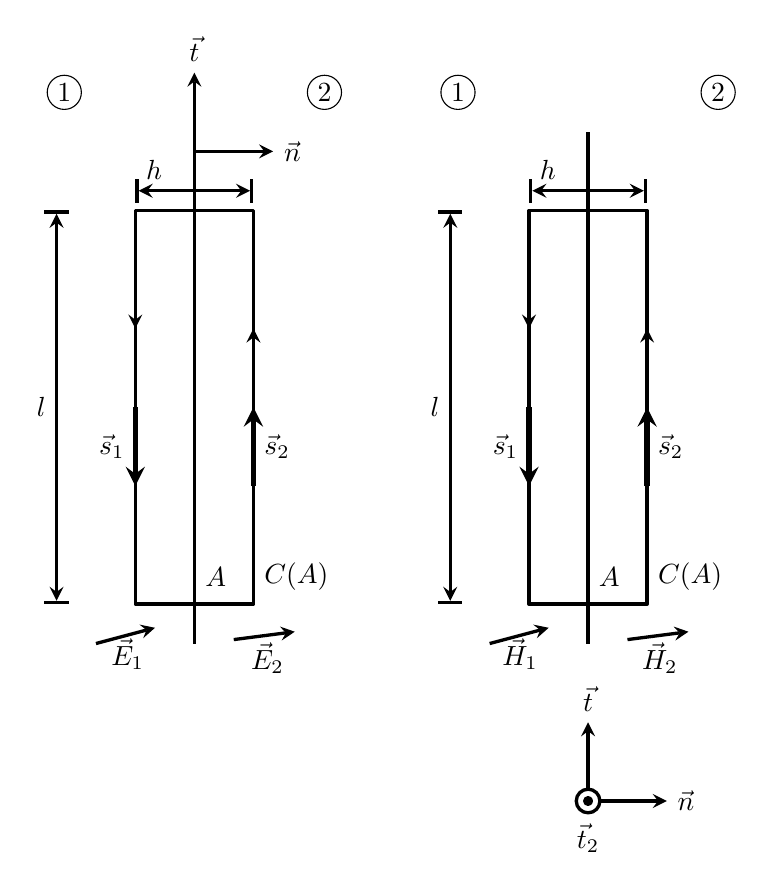
\begin{tikzpicture}[line width = 1.2pt, line join=round,x=0.5cm,y=0.5cm,>=stealth]
	% Mittellinie zeichnen
	\draw (0,-6) -- (0,7);
	% Schleife zeichnen
	\draw (-1.5,-5) rectangle (1.5,5);
	% Richtungen der Schleife
	\draw [->] (-1.5,3) -- (-1.5,2);
	\draw [->] (1.5,1) -- (1.5,2);
	% Vektoren für ds Zeichnen
	\draw [->,line width = 2pt] (-1.5,0) -- (-1.5,-2);
	\draw (-1.5,-1) node[anchor=east] {$\dd \vec{s}_1$};
	\draw [->,line width = 2pt] (1.5,-2) -- (1.5,0);
	\draw (1.5,-1) node[anchor=west] {$\dd \vec{s}_2$};
	% Breite der Schleife
	\draw [|<->|] (1.5,5.5) -- (-1.5,5.5) node[anchor=south west] {$ h $};
	% Höhe der Schleife
	\draw [|<->|] (-3.5,-5) -- (-3.5,5);
	\draw (-3.5,0) node[anchor=east] {$ l $};
	% Normalenvektor
	\draw [->] (0,6.5) -- (2,6.5) node[anchor=west] {$ \vec{n} $};
	% Tangentialvektor
	\draw [->] (0,6.5) -- (0,8.5) node[anchor=south] {$ \vec{t} $};
	% Flächenbezeichnung und Randbezeichnung
	\draw (0,-4.3) node[anchor=west] {$ A $};
	\draw (1.5,-4.3) node[anchor=west] {$ C(A) $};
	% elektrisches Feld
	\draw [->] (-2.5,-6) -- (-1,-5.6) node[anchor=north east] {$ \vec{E}_1 $};
	\draw [->] (1,-5.9) -- (2.55,-5.7) node[anchor=north east] {$ \vec{E}_2 $};
	% Definition der Seiten
	\draw (-4,8) node[anchor=west] {\tikz[baseline=(char.base)]{
			\node[shape=circle,draw,inner sep=1.5pt] (char) {1}}};
	\draw (4,8) node[anchor=east] {\tikz[baseline=(char.base)]{
			\node[shape=circle,draw,inner sep=1.5pt] (char) {2}}};
	% Mittellinie zeichnen
	\draw (10,-6) -- (10,7);
	% Schleife zeichnen
	\draw (8.5,-5) rectangle (11.5,5);
	% Richtungen der Schleife
	\draw [->] (8.5,3) -- (8.5,2);
	\draw [->] (11.5,1) -- (11.5,2);
	% Vektoren für ds Zeichnen
	\draw [->,line width = 2pt] (8.5,0) -- (8.5,-2);
	\draw (8.5,-1) node[anchor=east] {$\dd \vec{s}_1$};
	\draw [->,line width = 2pt] (11.5,-2) -- (11.5,0);
	\draw (11.5,-1) node[anchor=west] {$\dd \vec{s}_2$};
	% Breite der Schleife
	\draw [|<->|] (11.5,5.5) -- (8.5,5.5) node[anchor=south west] {$ h $};
	% Höhe der Schleife
	\draw [|<->|] (6.5,-5) -- (6.5,5);
	\draw (6.5,0) node[anchor=east] {$ l $};
	% Normalenvektor
	\draw [->] (10.3,-10) -- (12,-10) node[anchor=west] {$ \vec{n} $};
	% Tangentialvektor
	\draw [->] (10,-9.7) -- (10,-8) node[anchor=south] {$ \vec{t} $};
	% Tangentialvektor 2
	\draw (10,-10) circle (0.3);
	\filldraw (10,-10) circle (1.2pt);
	\draw (10,-10.3) node[anchor=north] {$ \vec{t}_2 $};
	% Flächenbezeichnung und Randbezeichnung
	\draw (10,-4.3) node[anchor=west] {$ A $};
	\draw (11.5,-4.3) node[anchor=west] {$ C(A) $};
	% magnetisches Feld
	\draw [->] (7.5,-6) -- (9,-5.6) node[anchor=north east] {$ \vec{H} _1 $};
	\draw [->] (11,-5.9) -- (12.55,-5.7) node[anchor=north east] {$ \vec{H} _2 $};
	% Definition der Seiten
	\draw (6,8) node[anchor=west] {\tikz[baseline=(char.base)]{
			\node[shape=circle,draw,inner sep=1.5pt] (char) {1}}};
	\draw (14,8) node[anchor=east] {\tikz[baseline=(char.base)]{
			\node[shape=circle,draw,inner sep=1.5pt] (char) {2}}};
\end{tikzpicture}